\documentclass[oneside,12pt]{article}          % ----- article

\input{../../Latex/inputs/loading_packages.tex}			% ----- Packages utiles
\input{../../Latex/inputs/preambule_general.tex}         	% ----- Préambule feuilles de TD
\input{../../Latex/inputs/mymacros.tex}                 % ----- Macros mathématiques
\input{../../Latex/inputs/mise_en_page.tex} 		   	% ----- Macros de mise en page

\fancyhead[L]{Séance \no 5}
\fancyhead[R]{T\up{ale} enseignement scientifique}            % En-tête droit
\fancyhead[C]{Suites numériques}
\fancyhf[CF]{\footnotesize{\etablissement}}                     % En-tête central
\fancyhf[LF]{M. Olivry}

\titlespacing{\section}{0pt}{2mm}{0pt}
\titlespacing{\subsection}{0pt}{5mm}{1mm}

\renewcommand{\thempfootnote}{\arabic{mpfootnote}}

%%%%%%%%%%%%%%%%%%%%%%%%%%%%%%%%%%%%%%%%%%%%%%%%%%%%%%%%%%%%%%%%%%%%%%%%%%%%%%%%%%%%%%%%%%%%%%%%%%%%%%%%%%%%%
%%%%%%%%%%%%%%%%%%%%%%%%%%%%%%%%%%%%%%%%%%%%%%%%%%%%%%%%%%%%%%%%%%%%%%%%%%%%%%%%%%%%%%%%%%%%%%%%%%%%%%%%%%%%%
%%%%%%%%%%%%%%%%%%%%%%%%%%%%%%%%%%%%%%%%%%%%%%%%%%%%%%%%%%%%%%%%%%%%%%%%%%%%%%%%%%%%%%%%%%%%%%%%%%%%%%%%%%%%%

\begin{document}

\section{Le modèle démographique de Thomas Robert Malthus}

\begin{minipage}{0.55\textwidth} \restoreskip
	Thomas Robert Malthus (1766-1834) est un économiste britannique et prêtre anglican qui s'est intéressé aux évolutions des populations. 
	
	 Il est surtout connu pour ses travaux sur les rapports entre les dynamiques de croissance de la population et la production, analysés dans une perspective \og pessimiste \fg, totalement opposée à l'idée smithienne\footnotemark[1] d'un équilibre harmonieux et stable. 
	 
	Il a notamment développé un modèle catastrophiste selon lequel une population ayant une croissance exponentielle se confronte, tôt ou tard, à la limite des ressources disponibles. 
	 
	Son nom a donné dans le langage courant un adjectif, \og malthusien \fg\, souvent négativement connoté (désignant un état d'esprit plutôt conservateur, opposé à l'investissement ou craignant la rareté), et une doctrine, le malthusianisme qui inclut une politique active de contrôle de la natalité pour maîtriser la croissance de la population.
\end{minipage} \hspace{5mm}
\begin{minipage}{0.4\textwidth}
	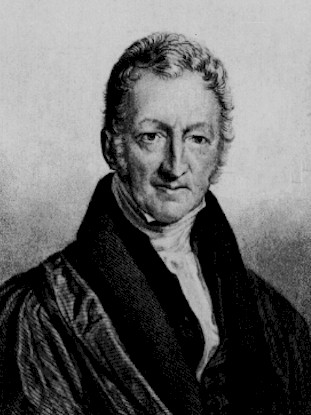
\includegraphics[scale=0.7]{malthus.jpg}
	\begin{center}
		Thomas Robert Malthus (1766 - 1834)
	\end{center}
\end{minipage}



\begin{tcolorbox}[
    enhanced , arc = 0pt , top = 4mm ,
    colback = white ,
    fonttitle = \bfseries , title = {Document \no 1 : Extrait de \og Essai sur le principe de population \fg} , boxed title style = {arc = 0pt} ,
    coltitle = black , colbacktitle = black!10 ,
    attach boxed title to top left = {xshift = 5mm , yshift = -4mm} ,
	]	

	{\ttfamily\itshape\restoreskip
	
	Selon la table d’Euler \footnotemark[2], si l’on se base sur une mortalité de 1 sur 36 et si naissances et	morts sont dans le rapport de 3 à 1, le chiffre de la population doublera en 12 années et 4/5. Ce n’est point là une simple supposition : c’est une réalité qui s’est produite plusieurs fois, et à de courts intervalles.
	
	Cependant, pour ne pas être taxé d’exagération, nous nous baserons sur l’accroissement le moins rapide, qui est garanti par la concordance de tous les témoignages. Nous pouvons être certains que lorsque la population n’est arrêtée par aucun obstacle, elle double tous les vingt-cinq ans, et croît ainsi de période en période [\ldots]
	}
	\begin{flushright}
	    \textbf{Thomas Robert Malthus , 1798}
	\end{flushright}
\end{tcolorbox}



\begin{tcolorbox}[
    enhanced , arc = 3pt , top = 4mm ,
    fonttitle = \bfseries , title = Questions sur le document \no 1  , boxed title style = {arc = 3pt} ,
    coltitle = black , colbacktitle = white ,
    attach boxed title to top left = {xshift = 5mm , yshift = -4mm} ,
	]

	\begin{enumerate}
		\item Selon les hypothèses faites par T.R. Malthus, quel est l’accroissement annuel de la population de la Grande-Bretagne ?
		\item Est-il correct d'affirmer que la population subira un doublement au bout de 12 années et $\frac{4}{5}$ ?
		\item En arrondissant à un doublement de population tous les 13 ans, donner une suite permettant de modéliser l'évolution de la population selon les hypothèses de T.R. Malthus.
	\end{enumerate}
\end{tcolorbox}



%%%%% Notes de bas de page %%%%%

\vfill
\footnotetext[1]{Adam Smith est connu dans l’histoire comme l'un des pères des sciences économiques modernes}
\footnotetext[2]{Leonhard Euler est un mathématicien et physicien suisse du XVIe siècle, souvent considéré comme l'un des plus grands mathématiciens de tous les temps.}

%%%%%%%%%%%%%%%%%%%%%%%%%%%%%%%%



\section{La croissance démographique face aux ressources disponibles}

\begin{tcolorbox}[
    enhanced , arc = 0pt , top = 4mm ,
    colback = white ,
    fonttitle = \bfseries , title = {Document \no 2 : Extrait de \og Essai sur le principe de population \fg} , boxed title style = {arc = 0pt} ,
    coltitle = black , colbacktitle = black!10 ,
    attach boxed title to top left = {xshift = 5mm , yshift = -4mm} ,
	]	

	{\ttfamily\itshape\restoreskip
	
	Comptons pour 11 millions la population de la Grande-Bretagne\footnotemark[3] et supposons que le produit actuel de son sol suffit pour la maintenir. Au bout de vingt-cinq ans, la population sera de 22 millions [\ldots]
	
	La race humaine croîtra selon la progression 1, 2, 4, 8, 16, 32, 64, 128, 256 \ldots tandis que les moyens de subsistance croîtront selon la progression 1, 2, 3, 4, 5, 6, 7, 8, 9 [\ldots]. Le rythme d’accroissement de la population, de période en période, l’emporte donc tellement sur celui de l’augmentation des subsistances que, pour maintenir le niveau et pour que la population existante trouve toujours des aliments en quantité suffisante, il faut qu’à chaque instant une loi supérieure fasse obstacle à son extension. 

	}
	\begin{flushright}
	    \textbf{Thomas Robert Malthus , 1798}
	\end{flushright}
\end{tcolorbox}


\begin{tcolorbox}[
    enhanced , arc = 3pt , top = 4mm ,
    fonttitle = \bfseries , title = Questions sur le document \no 2  , boxed title style = {arc = 3pt} ,
    coltitle = black , colbacktitle = white ,
    attach boxed title to top left = {xshift = 5mm , yshift = -4mm} ,
	]

	\begin{enumerate}
		\item Selon le raisonnement de T.R. Malthus, remplir le tableau ci-après consignant la population de la Grande-Bretagne entre les années 1798 et 1923 :
		
		\begin{center}
		\renewcommand{\arraystretch}{2}
			\begin{tabular}{| P{3cm} | P{1.75cm} | P{1.75cm} | P{1.75cm}| P{1.75cm} | P{1.75cm} | P{1.75cm} |}
			    \hline
			    \textbf{Année} & 1798 & 1823 & 1848 & 1873 & 1898 & 1923 \\
			    \hline
			    Population totale (en millions) & & & & & & \\
			    \hline
			    Population nourrie (en millions) & & & & & & \\
			    \hline
			    Proportion de la population nourrie (en \%) & & & & & & \\
			    \hline
			\end{tabular}
		\end{center}
		
		\item Toujours selon les mêmes hypothèses :
		\begin{enumerate}
			\item Quel semble être l'accroissement annuel de la population de la Grande-Bretagne ?
			\item Quel semble être l'accroissement annuel des moyens de subsistance de la Grande-Bretagne ?
		\end{enumerate}

		\item D'après le modèle de T.R. Malthus, en quelle année précisément la Grande-Bretagne ne pourra-t-elle plus subvenir aux besoin de sa population ?
	\end{enumerate}
\end{tcolorbox}



\vfill
\footnotetext[3]{Lors du premier recensement officiel en 1801, la population de la Grande-Bretagne s'élevait à 10 942 646 habitants.}



\section{Les limites du modèle}

\begin{tcolorbox}[
    enhanced , arc = 0pt , top = 4mm ,
    colback = white ,
    fonttitle = \bfseries , title = Document \no 3 : Évolution de la démographie en Grande-Bretagne, boxed title style = {arc = 0pt} ,
    coltitle = black , colbacktitle = black!10 ,
    attach boxed title to top left = {xshift = 5mm , yshift = -4mm} ,
	]
	
	\centering
	
	\begin{tikzpicture}
		\begin{axis}[
			axis lines = middle ,
		    width = 14cm , height = 8cm , xmin = 1960 , xmax = 2015 , ymin = 8, ymax =20 ,
		    xlabel={Année} ,
			xlabel style = {at = {(axis description cs:0.95,-0.08)} , anchor = north } ,
		    xtick = {1960,1965,...,2015},
		    xticklabel style = {/pgf/number format/fixed , /pgf/number format/1000 sep={}} ,
			ylabel={Taux (‰)} ,
			ylabel style = {at = {(axis description cs:-0.05,0.9)} , anchor = south , rotate = 90} ,
		    ytick = {8,10,12,14,16,18,20} ,
		    grid = major , xmajorgrids = false , ymajorgrids = true,
		    legend pos = north east,
		    legend style = {font = \small} ,
		    tick label style={font = \small} ,
		    label style = {font = \small} ,
		    enlarge x limits = 0.05,
			enlarge y limits = 0.05,
		]
		
		% Taux de natalité
		\addplot[newblue , line width = 2pt , mark=*]
		coordinates {
		    (1960,17.5)
		    (1965,18.3)
		    (1970,16.2)
		    (1975,12.4)
		    (1980,13.4)
		    (1985,13.3)
		    (1990,13.9)
		    (1995,12.6)
		    (2000,11.5)
		    (2005,12.0)
		    (2010,12.9)
		    (2015,11.9)
		};
		\addlegendentry{Taux de natalité}
		
		% Taux de mortalité
		\addplot[newred , line width = 2pt , mark = *]
		coordinates {
		    (1960,11.5)
		    (1965,11.6)
		    (1970,11.8)
		    (1975,11.8)
		    (1980,11.7)
		    (1985,11.9)
		    (1990,11.2)
		    (1995,11.1)
		    (2000,10.3)
		    (2005,9.6)
		    (2010,8.9)
		    (2015,9.2)
		};
		\addlegendentry{Taux de mortalité}
		
		\end{axis}
	\end{tikzpicture}
	
\end{tcolorbox}



\begin{tcolorbox}[
    enhanced , arc = 0pt , top = 4mm ,
    colback = white ,
    fonttitle = \bfseries , title = {Document \no 4 : Extrait de \og Essai de physique sociale \fg} , boxed title style = {arc = 0pt} ,
    coltitle = black , colbacktitle = black!10 ,
    attach boxed title to top left = {xshift = 5mm , yshift = -4mm} ,
	]	

	{\ttfamily\itshape\restoreskip
	
	Il paraît incontestable que la population croîtrait selon une progression géométrique, s’il ne se présentait aucun obstacle à son développement. Les moyens de subsistance ne se développent point aussi rapidement, et, selon Malthus, dans les circonstances les plus 	favorables à l’industrie, ils ne peuvent jamais augmenter plus vite que selon une progression arithmétique. Le grand obstacle à la population est donc le manque de nourriture, provenant de la différence des rapports que suivent ces deux quantités dans leurs accroissements respectifs. Quand une population, dans son développement, est parvenue au niveau de ses 	moyens de subsistance, elle doit s’arrêter à cette limite par la prévoyance des hommes ; ou si elle a le malheur de la franchir, elle s’y trouve forcément ramenée par un excès de mortalité.
	
	Les obstacles à la population peuvent donc être rangés sous deux chefs. Les uns agissent en prévenant l’accroissement de la population, et les autres en la détruisant à mesure qu'elle se forme. La somme des premiers compose ce que l’on peut appeler l’obstacle privatif ; celle des seconds l’obstacle destructif.
	}
	\begin{flushright}
	    \textbf{Adolphe Quételet , 1835}
	\end{flushright}
\end{tcolorbox}


\begin{tcolorbox}[
    enhanced , arc = 3pt , top = 4mm ,
    fonttitle = \bfseries , title = Questions sur les documents \no 3 \& \no 4  , boxed title style = {arc = 3pt} ,
    coltitle = black , colbacktitle = white ,
    attach boxed title to top left = {xshift = 5mm , yshift = -4mm} ,
	]

	\begin{enumerate}
		\item Quelle limite mathématique au modèle proposé par T.R. Malthus peut-on identifier sur le document \no 3 ?
		\item Quelles autres limites à ce modèle identifie A. Quételet dans son essai ?
	\end{enumerate}
\end{tcolorbox}



\newpage



\begin{tcolorbox}[
    enhanced , arc = 3pt , top = 4mm ,
    fonttitle = \bfseries , title = Je retiens  , boxed title style = {arc = 3pt} ,
    coltitle = black , colbacktitle = white ,
    attach boxed title to top left = {xshift = 5mm , yshift = -4mm} ,
	]
	\restoreskip
	
	Selon le modèle de T.R. Malthus \dotfill \\[5pt] \phantom{} \dotfill \\[5pt] \phantom{} \dotfill \\[5pt] \phantom{} \dotfill 

	\bigskip
	
	Le taux de mortalité est \dotfill \\[5pt] \phantom{} \dotfill \\[5pt] \phantom{} \dotfill \\[5pt] \phantom{} \dotfill
	
	\bigskip
	
	Le taux de natalité est \dotfill \\[5pt] \phantom{} \dotfill \\[5pt] \phantom{} \dotfill \\[5pt] \phantom{} \dotfill
	
	\bigskip
	
	Le modèle de T.R. Malthus ne permet pas de prédire correctement l'évolution de la population car
	
	\dotfill \\[5pt] \phantom{} \dotfill \\[5pt] \phantom{} \dotfill \\[5pt] \phantom{} \dotfill \\[5pt] \phantom{} \dotfill \\[5pt] \phantom{} \dotfill \\[5pt] \phantom{} \dotfill
\end{tcolorbox}




\end{document}	